\begin{frame}{Modelos de BRDFs}
    \begin{itemize}
        \item BRDF (Bidirectional Reflectance Distribution Function):  
              Função que descreve como a luz é refletida por uma superfície.
        \item Apresentaremos modelos clássicos de BRDFs:
        \begin{itemize}
            \item BRDF Pura Especular.
            \item BRDF Difusa Ideal.
            \item BRDF Brilhante.
            \item BRDF Retro-Refletora.
        \end{itemize}
    \end{itemize}
\end{frame}

% BRDF Pura Especular
\begin{frame}{BRDF Pura Especular}
    \begin{itemize}
        \item Superfície reflete luz apenas em uma direção.
        \item Segue a Lei da Reflexão:
        \[
        f(\omega_i, \omega_o) = k_s \cdot \delta(\omega_i - \omega_o)
        \]
        \item Materiais típicos: metal polido, vidro.
    \end{itemize}
    \begin{figure}[H]
        \centering
        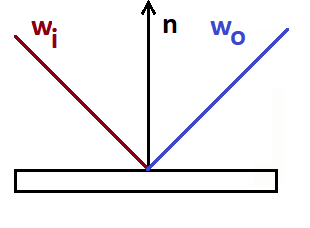
\includegraphics[scale=0.5]{./Imagens/specular-2d.png}
        \caption{\small Reflexão especular. Raio incidente em vermelho e raio refletido em azul.}
    \end{figure}
\end{frame}

% BRDF Difusa Ideal
\begin{frame}{BRDF Difusa Ideal}
    \begin{itemize}
        \item Reflexão uniforme em todas as direções.
        \item Função BRDF:
        \[
        f(\omega_i, \omega_o) = \frac{\rho_d}{\pi} \cdot \cos \theta
        \]
        \item Exemplos: tinta fosca, papel.
    \end{itemize}
    \begin{figure}[H]
        \centering
        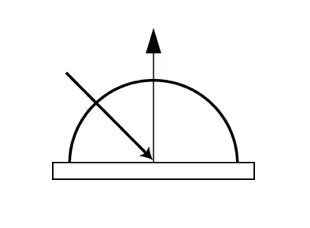
\includegraphics[scale=0.5]{./Imagens/diffuse-2d.png}
        \caption{\small Reflexão difusa. Raios refletidos independem do ângulo de entrada.}
    \end{figure}
\end{frame}

% BRDF Brilhante
\begin{frame}{BRDF Brilhante}
    \begin{itemize}
        \item Combina reflexões especulares e difusas.
        \item Modelo típico: Blinn-Phong.
    \end{itemize}
    \begin{figure}[H]
        \centering
        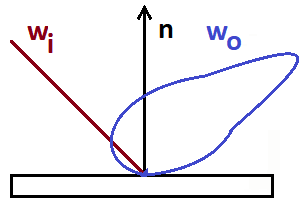
\includegraphics[scale=0.5]{./Imagens/glossy-2d.png}
        \caption{\small Reflexão \textit{glossy}.}
    \end{figure}
\end{frame}

% BRDF Retro-Refletora
\begin{frame}{BRDF Retro-Refletora}
    \begin{itemize}
        \item Redireciona a luz de volta à fonte.
        \item Utilizado em superfícies como placas de trânsito e sinais de segurança.
    \end{itemize}
    \begin{figure}[H]
        \centering
        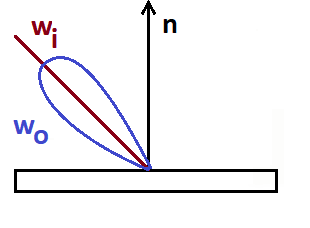
\includegraphics[scale=0.5]{./Imagens/retro-reflection-2d.png}
        \caption{\small Reflexão retro-refletora.}
    \end{figure}
\end{frame}

\begin{frame}{BRDF: Função de Refletância Bidirecional}
    \begin{itemize}
        \item BRDF (\( f \)) descreve como a luz reflete em diferentes direções:
        \[
        f(\omega_i, \omega_o) = \frac{dL_o(\omega_o)}{L_i(\omega_i) \cos(\theta_i) d\omega_i}
        \]
        \item Propriedades:
        \begin{enumerate}
            \item Positividade: \( f \geq 0 \).  
            \item Conservação de energia: \(\int_{\Omega} f \cos(\theta_i) d\omega_i \leq 1\).
            \item Reciprocidade de Helmholtz: \( f(\omega_i, \omega_o) = f(\omega_o, \omega_i) \).
        \end{enumerate}
    \end{itemize}
\end{frame}

\begin{frame}{Radiometria: Introdução}
    \begin{itemize}
        \item Estuda a interação da luz com superfícies na computação gráfica.
        \item Quantifica energia luminosa:
        \begin{itemize}
            \item Brilho da fonte de luz.
            \item Iluminação e refletância da superfície.
        \end{itemize}
        \item Fundamenta a renderização realista de cenas tridimensionais.
    \end{itemize}
\end{frame}

\begin{frame}{Energia Radiante $Q$}
    \begin{itemize}
        \item Quantifica a energia total dos fótons atingindo uma superfície.
        \item Fórmula:
        \[
            Q = \frac{hc}{\lambda}
        \]

        onde:
        \begin{itemize}
            \item \( h \): Constante de Planck.  
            \item \( c \): Velocidade da luz.  
            \item \( \lambda \): Comprimento de onda.  
        \end{itemize}
    \end{itemize}
\end{frame}

\begin{frame}{Fluxo Radiante e Irradiância}
    \begin{itemize}
        \item Fluxo Radiante: Energia por unidade de tempo (\( J/s \)):
        \[
            \phi = \frac{dQ}{dt} % \left[\text{J/s}\right]
        \]
        \item Irradiância: Fluxo radiante por unidade de área:
        \[
        E(p) = \frac{d\phi(p)}{dA} %  \left[ \frac{\text{J}} {s\cdot m^2} \right]
        \]
    \item Quantifica os impactos de fótons em uma superfície.\footnote{\footnotesize{Saber quantos fótons "tocam" uma superfície por segundo, é saber quão iluminado é aquela parte do objeto.}}
    \end{itemize}
\end{frame}

\begin{frame}{Radiância}
    Radiância (\( L \)): Fluxo radiante por unidade de área e ângulo sólido:
    \[
    L = \frac{d^2\Phi}{dA \, d\omega \cos(\theta)}
    \]
    Onde:
    \begin{itemize}
        \item \( d\omega \): Ângulo sólido (em sr).  
        \item \( \theta \): Ângulo entre direção de incidência e normal da superfície.
    \end{itemize}
\end{frame}



\begin{frame}{Visualização da Radiância}
    \begin{itemize}
        \item Radiância considera direção específica no hemisfério sobre a superfície.
    \end{itemize}

\begin{figure}[h]
        \caption{\label{radiance-img} \small Visualização da radiância em uma direção específica do hemisfério. }
            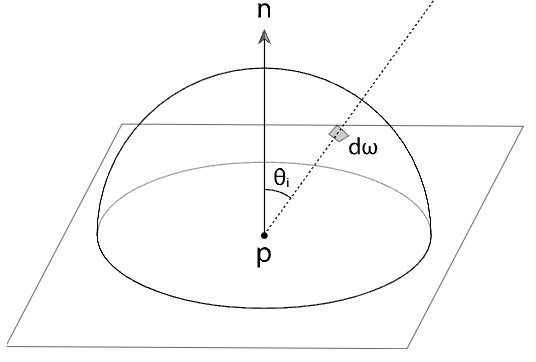
\includegraphics[scale=0.5]{./Imagens/irradiance_hemisphere.png}
  % \legend{ \small Fonte: \cite{pbr}. Adaptada.}
\end{figure}


\begin{figure}[h]
  \caption{\label{solid-angle} \small   Ângulo sólido s do objeto B visto pelo ponto p. }
            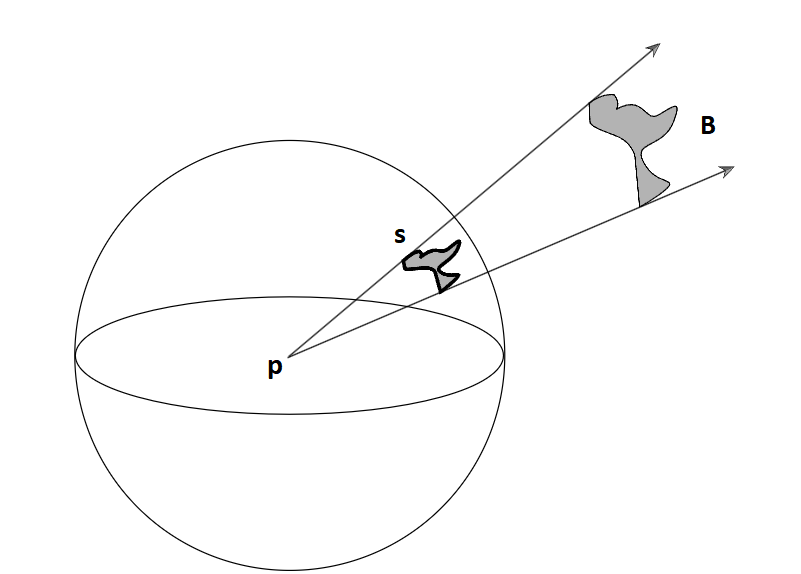
\includegraphics[scale=0.5]{./Imagens/solid_angle.png}
  % \legend{ \small Fonte: \cite{pbr}.}
\end{figure}
\end{frame}

\begin{frame}{Árvore SVG}
\end{frame}
